\begin{frame}[label=smr_goals]
    \frametitle{Goals of Meteor Radar}
    \begin{tikzpicture}[remember picture, overlay]
        \node[anchor=north east] at (current page.north east) {
            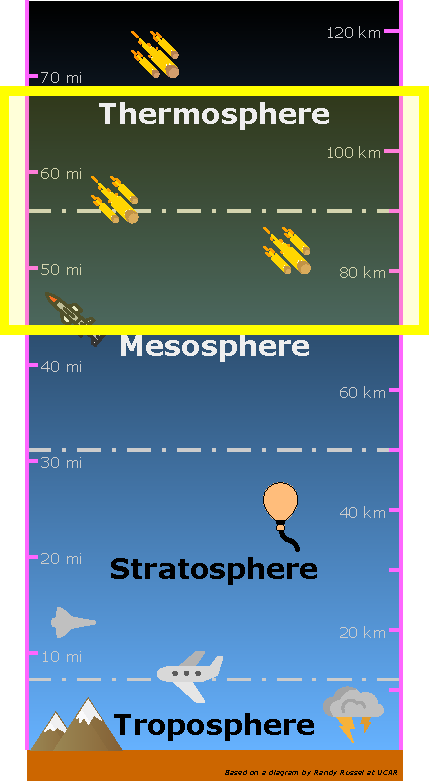
\includegraphics[height=\textheight]{img/atmos_layers.pdf}
        };
    \end{tikzpicture}
    \begin{columns}
        \begin{column}{0.8\textwidth}
            \uncover<2->{Can be used to study \alert{meteors}} \\ ~ \\ 
            \uncover<3->{I'm interested in the  \alert{Environment of the upper atmosphere}
            \begin{itemize}
                \item 70 - 110 km altitude 
                \item Wind, pressure, temperature
                \item Full field measurements over time
            \end{itemize}}
            \uncover<4->{Ultimate goal: \alert{Science!}
            \begin{itemize}
                \item Seasonal trends
                \item Energy transport 
                \item Inform atmospheric/circulation models 
            \end{itemize}}
            \uncover<5->{Why care? 
            \begin{itemize}
                \item Understand global environmental health
                \item Safety of near-Earth space economic activity
                \item Space domain awareness
            \end{itemize}}
            \centering
            \uncover<6->{\colorbox{yellow}{\textbf{No other way to \textit{densely} sample this region's environment!}}}
        \end{column}
        \begin{column}{0.2\textwidth}
            
        \end{column}
    \end{columns}
    \centering
\end{frame}
